\documentclass[10pt]{beamer}
\usepackage[utf8]{inputenc}

\usepackage[absolute,overlay]{textpos}
\usepackage{graphicx}
\usepackage{media9}

\mode<presentation> {
\usetheme{boxes} % When headline is wanted use Dresden theme instead
\usecolortheme{seagull}
\logo{
\includegraphics[height=1.5cm]{ku_logo_dk}}
\setbeamertemplate{footline}[frame number]
% \setbeamertemplate{footline}{
%   \hspace{1em}
%   \hfill
%   \insertframenumber/\inserttotalframenumber
%   \vspace{1em}
%   \hspace{1em}
%   
\includegraphics[height=2cm]{ku_logo_dk}
%   \hspace{1em}
% }
\setbeamertemplate{navigation symbols}{}
\setbeamertemplate{itemize items}[square]
}






%----------------------------------------------------------------------------------------
%	TITLE PAGE
%----------------------------------------------------------------------------------------

\title[Kickstart-kursus] % bottom of every slide
  {Kickstart-kursus i programmering 22} % title page

\author{\footnotesize{Daniel Spikol} \\
          \footnotesize{\texttt{ds@di.ku.dk}}}

\institute {DIKU \\ Københavns Universitet}

\date[16. august 2022]{16 august 2022}

\begin{document}
\begin{frame}[plain]
\titlepage
\end{frame}


\begin{frame}
   \frametitle{Pair Programming - Hello World!}
   	 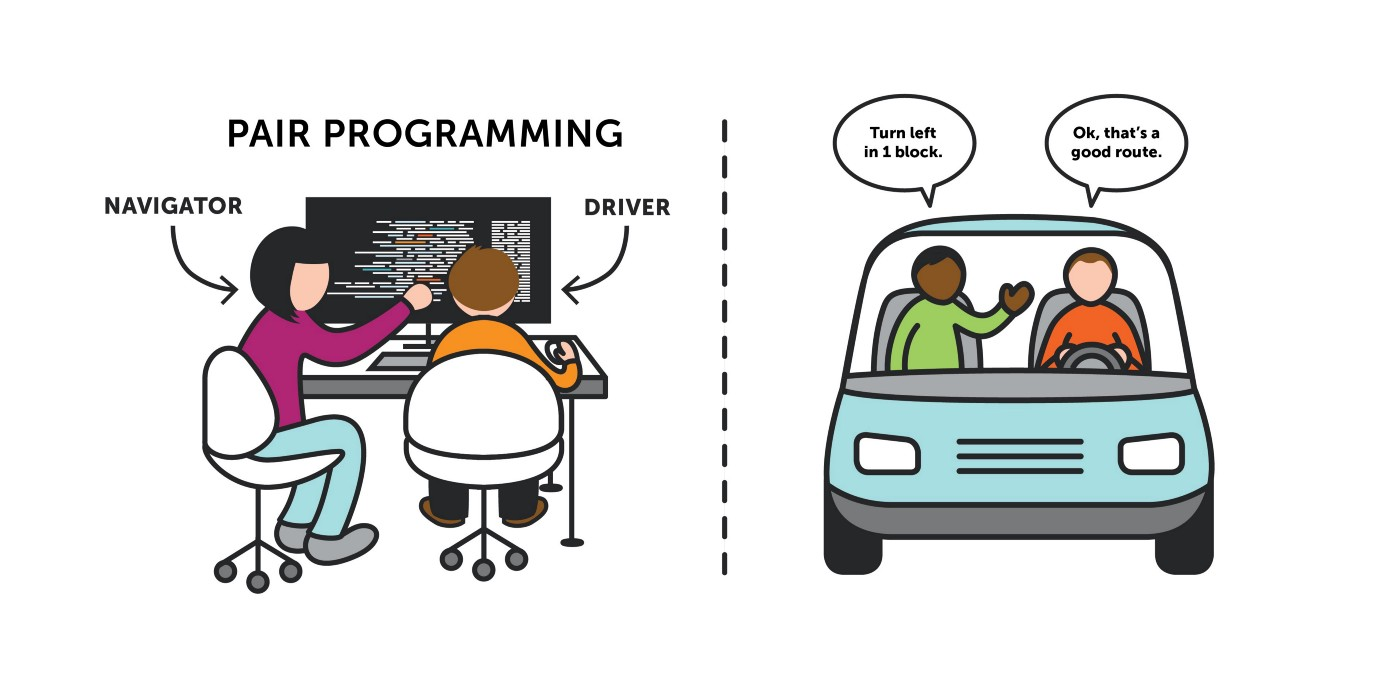
\includegraphics[height=8cm]{images/pairprog}
\end{frame}

\begin{frame}
   \frametitle{Recap from Yesterday}
   	\begin{itemize}
	\item Marshmallow Challenge - constant prototyping as problem-solving method
	\item Coordinate System 
	\item Drawing with Processing
	\item Variables
	\item Functions
	\end{itemize}
\end{frame}

\begin{frame}
   \frametitle{Processing History}
   	\begin{itemize}
	\item M.I.T. Media Lab Casey Reas \& Ben Fry
	\item Design By Numbers  - John Maeda
	\item Creative Programming
	\end{itemize}
\end{frame}

\begin{frame}
   \frametitle{Pair Programming - Hello World!}
   	 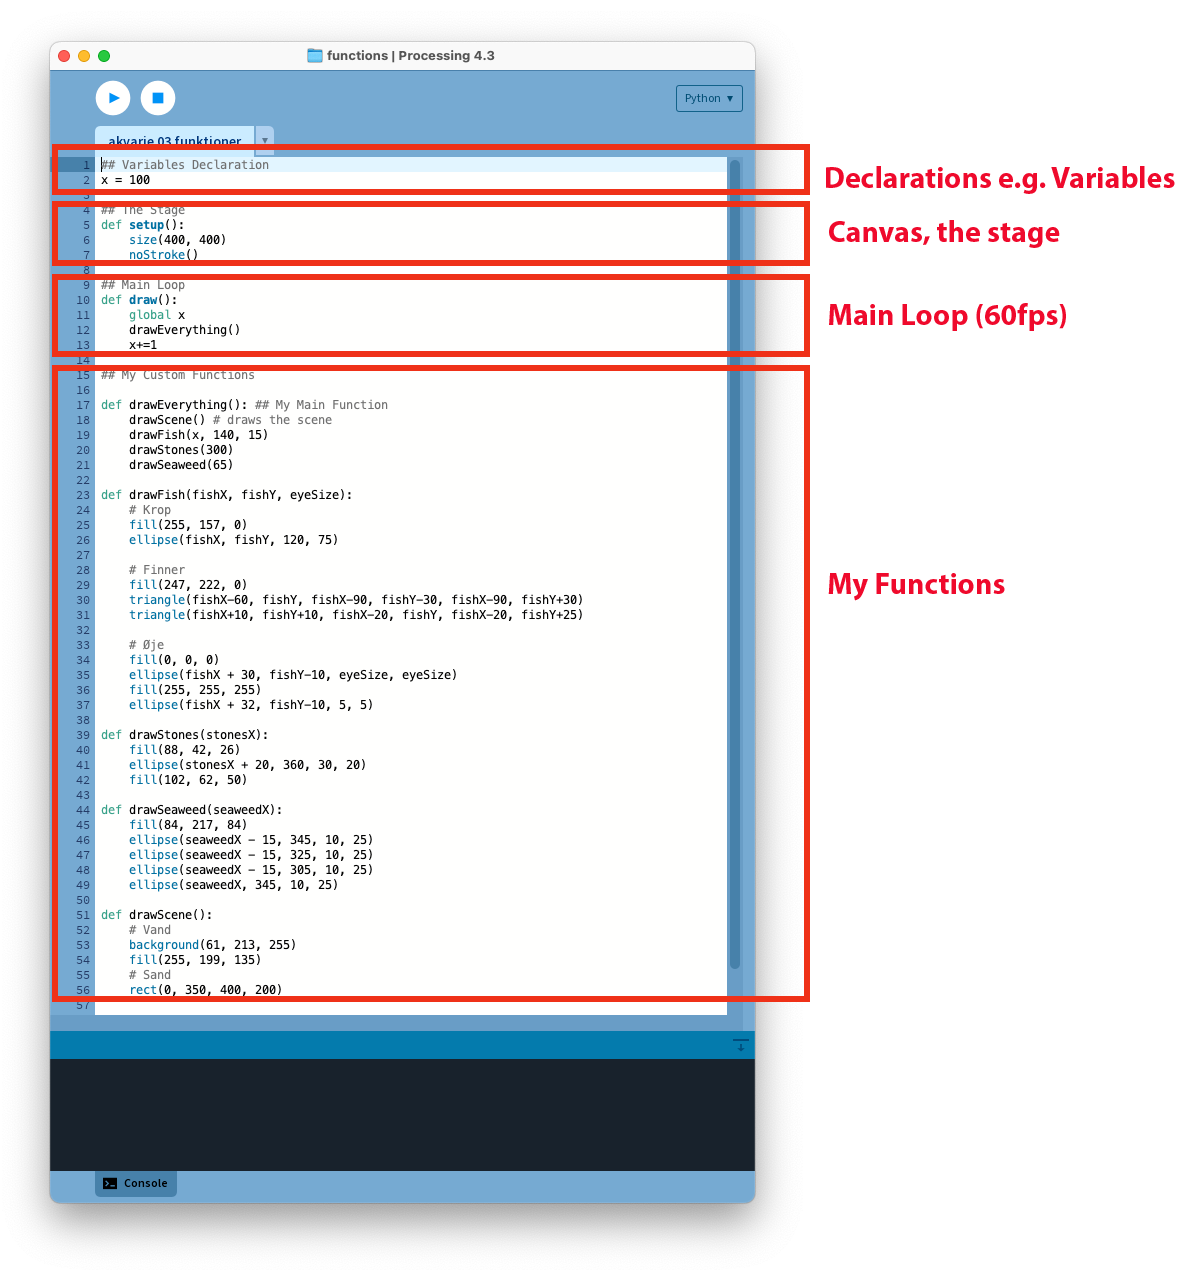
\includegraphics[height=8cm]{images/process}
\end{frame}



\begin{frame}
\frametitle{Todays Plan}
\begin{itemize}
\item Functions
\item Pair Programming
\item Animation
\end{itemize}
\end{frame}

\begin{frame}
  \frametitle{To hoveder er bedre end et}
  \framesubtitle{Pair programming}

  \begin{itemize}
  \item Par programmører udvikler software af højere kvalitet
  \item Lidt længere udviklingstid, men meget mindre tid brugt på at
    finde fejl bagefter.
  \item Hyggeligere og sjovere end at arbejde alene.
%  \item More enjoyable than working alone, pair programmers are happier programmers
%  \item SkaberCloser social connections
  \item Forbedret vidensdeling mellem programmørerne, mindre tid brugt
    på koordinering %Improved knowledge transfer
  \item Øget læring (og det er derfor I er her ikke?), man skiftes på
    en måde til at undervise hinanden
    % \item Enhanced learning
    % \item Taking turns being the teacher
  \item Ellers ikke udtalte kundskaber og vaner er udvekslet
%  \item Unspoken skills and habits are exchanged
  \end{itemize}
  

\end{frame}

\begin{frame}
  \frametitle{Pair programming i praksis}


 To programmører, en computer
    \begin{itemize}
    \item Driver - har hænder på rattet (tastaturet)
      og øjnene på vejen (skærmen)
    \item Navigator - har fokus på destinationen og
      hvordan vi kommer derhen
    \end{itemize}

~
    
Regler
\begin{itemize}
  \item Du må ikke være kommanderende overfor din partner
  \item Navigatoren må ikke røre musen eller tastaturet
  \item Driveren må ikke ignorere navigatoren
  \item I skal bytte roller ofte (fx hvert 20. minut)
  \item Forsøg at holde en samtale kørende
  \end{itemize}
 \end{frame}

\begin{frame}
  \frametitle{Samtaler mellem driver og navigator}
    \begin{itemize}
  \item God pair programmering er ikke uden kommunikation og snak. 
  \item Tal sammen i paret hele tiden om hvad der sker på
    skærmen. 
  \item Reflekter over det I har lavet og hvor I er på vej hen.
  \item Driveren fortæller hvad de er i gang med, hvad der sker.
  \item Navigatoren kommer med kommentarer, sørger for at de er i gang
    med det rigtige og fortæller hvad de skal nu og senere.
  \end{itemize}

  ~

  Eksempler:
  \begin{itemize}
  \item Driver: ``Nu opretter vi en ny funktion til at tegne en solsikke''
  \item Driver: ``Nu afprøver vi lige om XYZ virker, inden vi fortsætter.''
  \item Navigator: ``Hvordan kan det være du gør det?''
  \item Navigator: ``Kan du forklare hvad du er i gang med?''
  \end{itemize}
\end{frame}

\begin{frame}
  \frametitle{Recap}
    \begin{itemize}
    \item Pair Programming
  	\item Functions
	\item Animation
	\item How do you feel about pair programming?
\end{itemize}
\end{frame}

\begin{frame}
\frametitle{Tomorrow}
\begin{itemize}
\item Bbetingelser
\item Ideation og Brainstorming
\item Project ideas
\end{itemize}
\end{frame}

\end{document}